\documentclass[]{article}
\usepackage{lmodern}
\usepackage{amssymb,amsmath}
\usepackage{ifxetex,ifluatex}
\usepackage{fixltx2e} % provides \textsubscript
\ifnum 0\ifxetex 1\fi\ifluatex 1\fi=0 % if pdftex
  \usepackage[T1]{fontenc}
  \usepackage[utf8]{inputenc}
\else % if luatex or xelatex
  \ifxetex
    \usepackage{mathspec}
    \usepackage{xltxtra,xunicode}
  \else
    \usepackage{fontspec}
  \fi
  \defaultfontfeatures{Mapping=tex-text,Scale=MatchLowercase}
  \newcommand{\euro}{€}
\fi
% use upquote if available, for straight quotes in verbatim environments
\IfFileExists{upquote.sty}{\usepackage{upquote}}{}
% use microtype if available
\IfFileExists{microtype.sty}{%
\usepackage{microtype}
\UseMicrotypeSet[protrusion]{basicmath} % disable protrusion for tt fonts
}{}
\usepackage[margin=1in]{geometry}
\usepackage{color}
\usepackage{fancyvrb}
\newcommand{\VerbBar}{|}
\newcommand{\VERB}{\Verb[commandchars=\\\{\}]}
\DefineVerbatimEnvironment{Highlighting}{Verbatim}{commandchars=\\\{\}}
% Add ',fontsize=\small' for more characters per line
\usepackage{framed}
\definecolor{shadecolor}{RGB}{248,248,248}
\newenvironment{Shaded}{\begin{snugshade}}{\end{snugshade}}
\newcommand{\KeywordTok}[1]{\textcolor[rgb]{0.13,0.29,0.53}{\textbf{{#1}}}}
\newcommand{\DataTypeTok}[1]{\textcolor[rgb]{0.13,0.29,0.53}{{#1}}}
\newcommand{\DecValTok}[1]{\textcolor[rgb]{0.00,0.00,0.81}{{#1}}}
\newcommand{\BaseNTok}[1]{\textcolor[rgb]{0.00,0.00,0.81}{{#1}}}
\newcommand{\FloatTok}[1]{\textcolor[rgb]{0.00,0.00,0.81}{{#1}}}
\newcommand{\CharTok}[1]{\textcolor[rgb]{0.31,0.60,0.02}{{#1}}}
\newcommand{\StringTok}[1]{\textcolor[rgb]{0.31,0.60,0.02}{{#1}}}
\newcommand{\CommentTok}[1]{\textcolor[rgb]{0.56,0.35,0.01}{\textit{{#1}}}}
\newcommand{\OtherTok}[1]{\textcolor[rgb]{0.56,0.35,0.01}{{#1}}}
\newcommand{\AlertTok}[1]{\textcolor[rgb]{0.94,0.16,0.16}{{#1}}}
\newcommand{\FunctionTok}[1]{\textcolor[rgb]{0.00,0.00,0.00}{{#1}}}
\newcommand{\RegionMarkerTok}[1]{{#1}}
\newcommand{\ErrorTok}[1]{\textbf{{#1}}}
\newcommand{\NormalTok}[1]{{#1}}
\usepackage{graphicx}
\makeatletter
\def\maxwidth{\ifdim\Gin@nat@width>\linewidth\linewidth\else\Gin@nat@width\fi}
\def\maxheight{\ifdim\Gin@nat@height>\textheight\textheight\else\Gin@nat@height\fi}
\makeatother
% Scale images if necessary, so that they will not overflow the page
% margins by default, and it is still possible to overwrite the defaults
% using explicit options in \includegraphics[width, height, ...]{}
\setkeys{Gin}{width=\maxwidth,height=\maxheight,keepaspectratio}
\ifxetex
  \usepackage[setpagesize=false, % page size defined by xetex
              unicode=false, % unicode breaks when used with xetex
              xetex]{hyperref}
\else
  \usepackage[unicode=true]{hyperref}
\fi
\hypersetup{breaklinks=true,
            bookmarks=true,
            pdfauthor={},
            pdftitle={Anaquin TransQuin Report},
            colorlinks=true,
            citecolor=blue,
            urlcolor=blue,
            linkcolor=magenta,
            pdfborder={0 0 0}}
\urlstyle{same}  % don't use monospace font for urls
\setlength{\parindent}{0pt}
\setlength{\parskip}{6pt plus 2pt minus 1pt}
\setlength{\emergencystretch}{3em}  % prevent overfull lines
\setcounter{secnumdepth}{0}

%%% Use protect on footnotes to avoid problems with footnotes in titles
\let\rmarkdownfootnote\footnote%
\def\footnote{\protect\rmarkdownfootnote}

%%% Change title format to be more compact
\usepackage{titling}

% Create subtitle command for use in maketitle
\newcommand{\subtitle}[1]{
  \posttitle{
    \begin{center}\large#1\end{center}
    }
}

\setlength{\droptitle}{-2em}
  \title{Anaquin TransQuin Report}
  \pretitle{\vspace{\droptitle}\centering\huge}
  \posttitle{\par}
  \author{}
  \preauthor{}\postauthor{}
  \date{}
  \predate{}\postdate{}

\usepackage{graphicx}


\begin{document}

\maketitle


\section{Read Alignment}\label{read-alignment}

\begin{Shaded}
\begin{Highlighting}[]
\NormalTok{Summary for dataset:}\StringTok{ }\NormalTok{K_RMXA1v2.accepted_hits.sorted.bam}

   \NormalTok{Unmapped:}\StringTok{   }\DecValTok{0} \NormalTok{reads}
   \NormalTok{Experiment:}\StringTok{ }\DecValTok{36484961} \NormalTok{(}\FloatTok{76.13}\NormalTok{%) reads}
   \NormalTok{Synthetic:}\StringTok{  }\DecValTok{11440146} \NormalTok{(}\FloatTok{23.87}\NormalTok{%) reads}

   \NormalTok{Reference:}\StringTok{  }\DecValTok{1190} \NormalTok{exons}
   \NormalTok{Reference:}\StringTok{  }\DecValTok{1028} \NormalTok{introns}
   \NormalTok{Reference:}\StringTok{  }\DecValTok{149219} \NormalTok{bases}

   \NormalTok{Query:}\StringTok{      }\DecValTok{84739030} \NormalTok{exons}
   \NormalTok{Query:}\StringTok{      }\DecValTok{27056077} \NormalTok{introns}
   \NormalTok{Query:}\StringTok{      }\DecValTok{153438} \NormalTok{bases}

   \NormalTok{Dilution:}\StringTok{   }\FloatTok{0.238709}

   \NormalTok{**}\ErrorTok{*}
\StringTok{   }\ErrorTok{***}\StringTok{ }\NormalTok{The following statistics are computed at the exon, intron and base level.}
   \NormalTok{**}\ErrorTok{*}
\StringTok{   }\ErrorTok{***}\StringTok{ }\NormalTok{Exon level is defined by performance per exon. An alignment that}
   \NormalTok{**}\ErrorTok{*}\StringTok{ }\NormalTok{is not mapped entirely within an exon is considered as a FP. The}
   \NormalTok{**}\ErrorTok{*}\StringTok{ }\NormalTok{intron level is similar.}
   \NormalTok{**}\ErrorTok{*}
\StringTok{   }\ErrorTok{***}\StringTok{ }\NormalTok{Base level is defined by performance per nucleotide. A partial}
   \NormalTok{**}\ErrorTok{*}\StringTok{ }\NormalTok{mapped read will have FP and TP.}
   \NormalTok{**}\ErrorTok{*}

\StringTok{   }\NormalTok{--------------------}\StringTok{ }\NormalTok{Exon level --------------------}

\StringTok{   }\NormalTok{Sensitivity:}\StringTok{ }\FloatTok{0.997479}
   \NormalTok{Specificity:}\StringTok{ }\FloatTok{0.984404}
   \NormalTok{Detection:}\StringTok{   }\FloatTok{0.0590086} \NormalTok{(R2_33)}

   \NormalTok{--------------------}\StringTok{ }\NormalTok{Intron level --------------------}

\StringTok{   }\NormalTok{Sensitivity:}\StringTok{ }\FloatTok{0.993191}
   \NormalTok{Specificity:}\StringTok{ }\DecValTok{1}
   \NormalTok{Detection:}\StringTok{   }\FloatTok{0.0590086} \NormalTok{(R2_33)}

   \NormalTok{--------------------}\StringTok{ }\NormalTok{Base level --------------------}

\StringTok{   }\NormalTok{Sensitivity:}\StringTok{ }\FloatTok{0.703341}
   \NormalTok{Specificity:}\StringTok{ }\DecValTok{1}
   \NormalTok{Detection:}\StringTok{   }\FloatTok{0.0590086} \NormalTok{(R2_33)}
\end{Highlighting}
\end{Shaded}

\section{Transctiptome Assembly}\label{transctiptome-assembly}

\begin{Shaded}
\begin{Highlighting}[]
\NormalTok{Summary for dataset:}\StringTok{ }\NormalTok{transcripts.gtf}

   \NormalTok{Experiment:}\StringTok{ }\DecValTok{1897} \NormalTok{features}
   \NormalTok{Synthetic:}\StringTok{  }\DecValTok{799} \NormalTok{features}

   \NormalTok{Reference:}\StringTok{  }\DecValTok{162} \NormalTok{exons}
   \NormalTok{Reference:}\StringTok{  }\DecValTok{1028} \NormalTok{introns}

   \NormalTok{**}\ErrorTok{*}
\StringTok{   }\ErrorTok{***}\StringTok{ }\NormalTok{The following statistics are computed for exact and fuzzy.}
   \NormalTok{**}\ErrorTok{*}
\StringTok{   }\ErrorTok{***}\StringTok{ }\NormalTok{The fuzzy level is }\DecValTok{10} \NormalTok{nucleotides.}
   \NormalTok{**}\ErrorTok{*}

\StringTok{   }\NormalTok{--------------------}\StringTok{ }\NormalTok{Exon level --------------------}

\StringTok{   }\NormalTok{Sensitivity:}\StringTok{ }\FloatTok{0.547018} \NormalTok{(}\FloatTok{0.566514}\NormalTok{)}
   \NormalTok{Specificity:}\StringTok{ }\FloatTok{0.952096} \NormalTok{(}\FloatTok{0.986028}\NormalTok{)}
   \NormalTok{Detection:}\StringTok{   }\FloatTok{0.015736} \NormalTok{(R2_72_1)}

   \NormalTok{--------------------}\StringTok{ }\NormalTok{Intron level --------------------}

\StringTok{   }\NormalTok{Sensitivity:}\StringTok{ }\FloatTok{0.521164} \NormalTok{(}\FloatTok{0.52381}\NormalTok{)}
   \NormalTok{Specificity:}\StringTok{ }\FloatTok{0.987469} \NormalTok{(}\FloatTok{0.992481}\NormalTok{)}
   \NormalTok{Detection:}\StringTok{   }\FloatTok{0.015736} \NormalTok{(R2_72_1)}

   \NormalTok{--------------------}\StringTok{ }\NormalTok{Base level --------------------}

\StringTok{   }\NormalTok{Sensitivity:}\StringTok{ }\FloatTok{0.570883}
   \NormalTok{Specificity:}\StringTok{ }\FloatTok{0.906859}
   \NormalTok{Detection:}\StringTok{   }\FloatTok{0.472069} \NormalTok{(R2_28)}

   \NormalTok{--------------------}\StringTok{ }\NormalTok{Intron Chain level --------------------}

\StringTok{   }\NormalTok{Sensitivity:}\StringTok{ }\FloatTok{0.394904} \NormalTok{(}\FloatTok{0.414013}\NormalTok{)}
   \NormalTok{Specificity:}\StringTok{ }\FloatTok{0.681319} \NormalTok{(}\FloatTok{0.714286}\NormalTok{)}

   \NormalTok{--------------------}\StringTok{ }\NormalTok{Transcript level --------------------}

\StringTok{   }\NormalTok{Sensitivity:}\StringTok{ }\FloatTok{0.393939} \NormalTok{(}\FloatTok{0.393939}\NormalTok{)}
   \NormalTok{Specificity:}\StringTok{ }\FloatTok{0.555556} \NormalTok{(}\FloatTok{0.555556}\NormalTok{)}

   \NormalTok{Missing exons:}\StringTok{ }\DecValTok{385}\NormalTok{/}\DecValTok{872} \NormalTok{(}\FloatTok{0.441514}\NormalTok{)}
   \NormalTok{Missing introns:}\StringTok{ }\DecValTok{324}\NormalTok{/}\DecValTok{756} \NormalTok{(}\FloatTok{0.428571}\NormalTok{)}

   \NormalTok{Novel exons:}\StringTok{ }\DecValTok{23}\NormalTok{/}\DecValTok{501} \NormalTok{(}\FloatTok{0.0459082}\NormalTok{)}
   \NormalTok{Novel introns:}\StringTok{ }\DecValTok{1}\NormalTok{/}\DecValTok{399} \NormalTok{(}\FloatTok{0.00250627}\NormalTok{)}
\end{Highlighting}
\end{Shaded}

\section{Expression Analysis (Genes)}\label{expression-analysis-genes}

\begin{Shaded}
\begin{Highlighting}[]
\NormalTok{Summary for dataset:}\StringTok{ }\NormalTok{stringout_sub0.01_guided_B/stringout_sub0.01_guided_genes.txt}

   \NormalTok{Experiment:}\StringTok{  }\DecValTok{601} \NormalTok{genes}
   \NormalTok{Synthetic:}\StringTok{   }\DecValTok{68} \NormalTok{genes}

   \NormalTok{Reference:}\StringTok{   }\DecValTok{76} \NormalTok{genes}
   \NormalTok{Detected:}\StringTok{    }\DecValTok{68} \NormalTok{genes}

   \NormalTok{**}\ErrorTok{*}
\StringTok{   }\ErrorTok{***}\StringTok{ }\NormalTok{Detection Limits}
   \NormalTok{**}\ErrorTok{*}

\StringTok{   }\NormalTok{Absolute:}\StringTok{    }\FloatTok{0.0590086} \NormalTok{(attomol/ul) (R2_33)}

   \NormalTok{Correlation:}\StringTok{ }\FloatTok{0.951391}
   \NormalTok{Slope:}\StringTok{       }\FloatTok{5.17238}
   \NormalTok{R2:}\StringTok{          }\FloatTok{0.905145}
   \NormalTok{F-statistic:}\StringTok{ }\FloatTok{610.716}
   \NormalTok{P-value:}\StringTok{     }\DecValTok{0}
   \NormalTok{SSM:}\StringTok{         }\FloatTok{8.78529e+10}\NormalTok{, DF:}\StringTok{ }\DecValTok{1}
   \NormalTok{SSE:}\StringTok{         }\FloatTok{9.20654e+09}\NormalTok{, DF:}\StringTok{ }\DecValTok{64}
   \NormalTok{SST:}\StringTok{         }\FloatTok{9.70595e+10}\NormalTok{, DF:}\StringTok{ }\DecValTok{65}

   \NormalTok{**}\ErrorTok{*}
\StringTok{   }\ErrorTok{***}\StringTok{ }\NormalTok{The following statistics are computed on the log2 scale.}
   \NormalTok{**}\ErrorTok{*}
\StringTok{   }\ErrorTok{***}\StringTok{   }\NormalTok{Eg:}\StringTok{ }\NormalTok{If the data points }\KeywordTok{are} \NormalTok{(}\DecValTok{1}\NormalTok{,}\DecValTok{1}\NormalTok{), (}\DecValTok{2}\NormalTok{,}\DecValTok{2}\NormalTok{). The correlation will}
   \NormalTok{**}\ErrorTok{*}\StringTok{       }\NormalTok{be computed }\KeywordTok{on} \NormalTok{(}\KeywordTok{log2}\NormalTok{(}\DecValTok{1}\NormalTok{), }\KeywordTok{log2}\NormalTok{(}\DecValTok{1}\NormalTok{)), (}\KeywordTok{log2}\NormalTok{(}\DecValTok{2}\NormalTok{), }\KeywordTok{log2}\NormalTok{(}\DecValTok{2}\NormalTok{))}\ErrorTok{)}
   \NormalTok{**}\ErrorTok{*}

\StringTok{   }\NormalTok{Correlation:}\StringTok{ }\FloatTok{0.960584}
   \NormalTok{Slope:}\StringTok{       }\FloatTok{0.944504}
   \NormalTok{R2:}\StringTok{          }\FloatTok{0.922722}
   \NormalTok{F-statistic:}\StringTok{ }\FloatTok{764.178}
   \NormalTok{P-value:}\StringTok{     }\DecValTok{0}
   \NormalTok{SSM:}\StringTok{         }\FloatTok{1518.12}\NormalTok{, DF:}\StringTok{ }\DecValTok{1}
   \NormalTok{SSE:}\StringTok{         }\FloatTok{127.143}\NormalTok{, DF:}\StringTok{ }\DecValTok{64}
   \NormalTok{SST:}\StringTok{         }\FloatTok{1645.26}\NormalTok{, DF:}\StringTok{ }\DecValTok{65}
\end{Highlighting}
\end{Shaded}

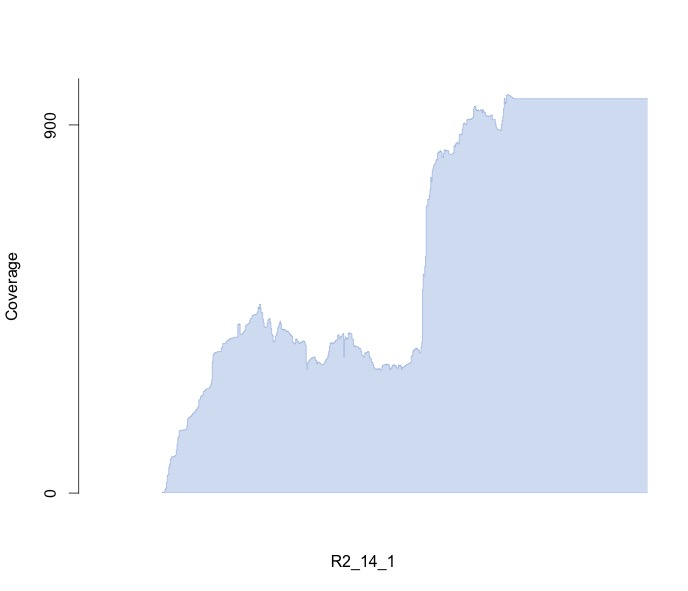
\includegraphics{1.jpeg}

\pagebreak

\section{Expression Analysis
(Isoforms)}\label{expression-analysis-isoforms}

\begin{Shaded}
\begin{Highlighting}[]
\NormalTok{Summary for dataset:}\StringTok{ }\NormalTok{stringout_sub0.01_guided_B/t_data.ctab}

   \NormalTok{Experiment:}\StringTok{  }\DecValTok{0} \NormalTok{isoforms}
   \NormalTok{Synthetic:}\StringTok{   }\DecValTok{164} \NormalTok{isoforms}

   \NormalTok{Reference:}\StringTok{   }\DecValTok{162} \NormalTok{isoforms}
   \NormalTok{Detected:}\StringTok{    }\DecValTok{162} \NormalTok{isoforms}

   \NormalTok{**}\ErrorTok{*}
\StringTok{   }\ErrorTok{***}\StringTok{ }\NormalTok{Detection Limits}
   \NormalTok{**}\ErrorTok{*}

\StringTok{   }\NormalTok{Absolute:}\StringTok{    }\FloatTok{0.00393391} \NormalTok{(attomol/ul) (R2_38_1)}

   \NormalTok{Correlation:}\StringTok{ }\FloatTok{0.945312}
   \NormalTok{Slope:}\StringTok{       }\FloatTok{5.26846}
   \NormalTok{R2:}\StringTok{          }\FloatTok{0.893614}
   \NormalTok{F-statistic:}\StringTok{ }\FloatTok{520.784}
   \NormalTok{P-value:}\StringTok{     }\DecValTok{0}
   \NormalTok{SSM:}\StringTok{         }\FloatTok{7.01119e+10}\NormalTok{, DF:}\StringTok{ }\DecValTok{1}
   \NormalTok{SSE:}\StringTok{         }\FloatTok{8.34691e+09}\NormalTok{, DF:}\StringTok{ }\DecValTok{62}
   \NormalTok{SST:}\StringTok{         }\FloatTok{7.84588e+10}\NormalTok{, DF:}\StringTok{ }\DecValTok{63}

   \NormalTok{**}\ErrorTok{*}
\StringTok{   }\ErrorTok{***}\StringTok{ }\NormalTok{The following statistics are computed on the log2 scale.}
   \NormalTok{**}\ErrorTok{*}
\StringTok{   }\ErrorTok{***}\StringTok{   }\NormalTok{Eg:}\StringTok{ }\NormalTok{If the data points }\KeywordTok{are} \NormalTok{(}\DecValTok{1}\NormalTok{,}\DecValTok{1}\NormalTok{), (}\DecValTok{2}\NormalTok{,}\DecValTok{2}\NormalTok{). The correlation will}
   \NormalTok{**}\ErrorTok{*}\StringTok{       }\NormalTok{be computed }\KeywordTok{on} \NormalTok{(}\KeywordTok{log2}\NormalTok{(}\DecValTok{1}\NormalTok{), }\KeywordTok{log2}\NormalTok{(}\DecValTok{1}\NormalTok{)), (}\KeywordTok{log2}\NormalTok{(}\DecValTok{2}\NormalTok{), }\KeywordTok{log2}\NormalTok{(}\DecValTok{2}\NormalTok{))}\ErrorTok{)}
   \NormalTok{**}\ErrorTok{*}

\StringTok{   }\NormalTok{Correlation:}\StringTok{ }\FloatTok{0.927843}
   \NormalTok{Slope:}\StringTok{       }\FloatTok{0.894364}
   \NormalTok{R2:}\StringTok{          }\FloatTok{0.860892}
   \NormalTok{F-statistic:}\StringTok{ }\FloatTok{383.697}
   \NormalTok{P-value:}\StringTok{     }\DecValTok{0}
   \NormalTok{SSM:}\StringTok{         }\FloatTok{783.229}\NormalTok{, DF:}\StringTok{ }\DecValTok{1}
   \NormalTok{SSE:}\StringTok{         }\FloatTok{126.559}\NormalTok{, DF:}\StringTok{ }\DecValTok{62}
   \NormalTok{SST:}\StringTok{         }\FloatTok{909.787}\NormalTok{, DF:}\StringTok{ }\DecValTok{63}
\end{Highlighting}
\end{Shaded}

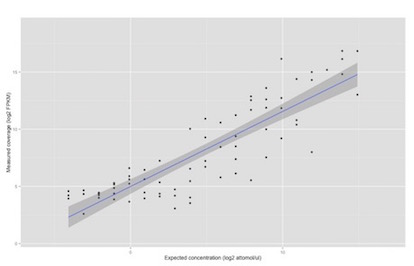
\includegraphics{2.jpeg}

\pagebreak

\section{Differential Analysis
(Genes)}\label{differential-analysis-genes}

\begin{Shaded}
\begin{Highlighting}[]
\NormalTok{Summary for dataset:}\StringTok{ }\NormalTok{gene_exp.diff}

   \NormalTok{Experiment:}\StringTok{  }\DecValTok{9682} \NormalTok{genes}
   \NormalTok{Synthetic:}\StringTok{   }\DecValTok{67} \NormalTok{genes}

   \NormalTok{Reference:}\StringTok{   }\DecValTok{76} \NormalTok{genes}
   \NormalTok{Detected:}\StringTok{    }\DecValTok{65} \NormalTok{genes}

   \NormalTok{**}\ErrorTok{*}
\StringTok{   }\ErrorTok{***}\StringTok{ }\NormalTok{Detection Limits}
   \NormalTok{**}\ErrorTok{*}

\StringTok{   }\NormalTok{Absolute:}\StringTok{    }\FloatTok{0.0590086} \NormalTok{(attomol/ul) (R2_33)}

   \NormalTok{Correlation:}\StringTok{ }\FloatTok{0.56272}
   \NormalTok{Slope:}\StringTok{       }\FloatTok{0.411349}
   \NormalTok{R2:}\StringTok{          }\FloatTok{0.316654}
   \NormalTok{F-statistic:}\StringTok{ }\FloatTok{29.1934}
   \NormalTok{P-value:}\StringTok{     }\FloatTok{1.06667e-06}
   \NormalTok{SSM:}\StringTok{         }\FloatTok{244.21}\NormalTok{, DF:}\StringTok{ }\DecValTok{1}
   \NormalTok{SSE:}\StringTok{         }\FloatTok{527.011}\NormalTok{, DF:}\StringTok{ }\DecValTok{63}
   \NormalTok{SST:}\StringTok{         }\FloatTok{771.221}\NormalTok{, DF:}\StringTok{ }\DecValTok{64}

   \NormalTok{**}\ErrorTok{*}
\StringTok{   }\ErrorTok{***}\StringTok{ }\NormalTok{The following statistics are computed on the log2 scale.}
   \NormalTok{**}\ErrorTok{*}
\StringTok{   }\ErrorTok{***}\StringTok{   }\NormalTok{Eg:}\StringTok{ }\NormalTok{If the data points }\KeywordTok{are} \NormalTok{(}\DecValTok{1}\NormalTok{,}\DecValTok{1}\NormalTok{), (}\DecValTok{2}\NormalTok{,}\DecValTok{2}\NormalTok{). The correlation will}
   \NormalTok{**}\ErrorTok{*}\StringTok{       }\NormalTok{be computed }\KeywordTok{on} \NormalTok{(}\KeywordTok{log2}\NormalTok{(}\DecValTok{1}\NormalTok{), }\KeywordTok{log2}\NormalTok{(}\DecValTok{1}\NormalTok{)), (}\KeywordTok{log2}\NormalTok{(}\DecValTok{2}\NormalTok{), }\KeywordTok{log2}\NormalTok{(}\DecValTok{2}\NormalTok{))}\ErrorTok{)}
   \NormalTok{**}\ErrorTok{*}

\StringTok{   }\NormalTok{Correlation:}\StringTok{ }\FloatTok{0.769414}
   \NormalTok{Slope:}\StringTok{       }\FloatTok{0.545994}
   \NormalTok{R2:}\StringTok{          }\FloatTok{0.591998}
   \NormalTok{F-statistic:}\StringTok{ }\FloatTok{91.4108}
   \NormalTok{P-value:}\StringTok{     }\FloatTok{7.00551e-14}
   \NormalTok{SSM:}\StringTok{         }\FloatTok{116.382}\NormalTok{, DF:}\StringTok{ }\DecValTok{1}
   \NormalTok{SSE:}\StringTok{         }\FloatTok{80.21}\NormalTok{, DF:}\StringTok{ }\DecValTok{63}
   \NormalTok{SST:}\StringTok{         }\FloatTok{196.592}\NormalTok{, DF:}\StringTok{ }\DecValTok{64}
\end{Highlighting}
\end{Shaded}

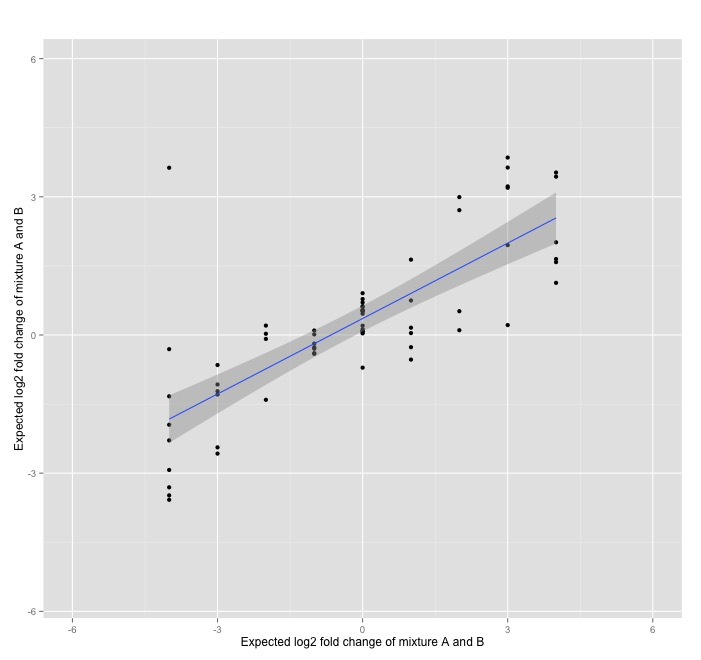
\includegraphics{4.jpeg}

\pagebreak

\section{Differential Analysis
(Isoforms)}\label{differential-analysis-isoforms}

\begin{Shaded}
\begin{Highlighting}[]
\NormalTok{Summary for dataset:}\StringTok{ }\NormalTok{gene_exp.diff}

   \NormalTok{Experiment:}\StringTok{  }\DecValTok{9682} \NormalTok{genes}
   \NormalTok{Synthetic:}\StringTok{   }\DecValTok{67} \NormalTok{genes}

   \NormalTok{Reference:}\StringTok{   }\DecValTok{76} \NormalTok{genes}
   \NormalTok{Detected:}\StringTok{    }\DecValTok{65} \NormalTok{genes}

   \NormalTok{**}\ErrorTok{*}
\StringTok{   }\ErrorTok{***}\StringTok{ }\NormalTok{Detection Limits}
   \NormalTok{**}\ErrorTok{*}

\StringTok{   }\NormalTok{Absolute:}\StringTok{    }\FloatTok{0.0590086} \NormalTok{(attomol/ul) (R2_33)}

   \NormalTok{Correlation:}\StringTok{ }\FloatTok{0.56272}
   \NormalTok{Slope:}\StringTok{       }\FloatTok{0.411349}
   \NormalTok{R2:}\StringTok{          }\FloatTok{0.316654}
   \NormalTok{F-statistic:}\StringTok{ }\FloatTok{29.1934}
   \NormalTok{P-value:}\StringTok{     }\FloatTok{1.06667e-06}
   \NormalTok{SSM:}\StringTok{         }\FloatTok{244.21}\NormalTok{, DF:}\StringTok{ }\DecValTok{1}
   \NormalTok{SSE:}\StringTok{         }\FloatTok{527.011}\NormalTok{, DF:}\StringTok{ }\DecValTok{63}
   \NormalTok{SST:}\StringTok{         }\FloatTok{771.221}\NormalTok{, DF:}\StringTok{ }\DecValTok{64}

   \NormalTok{**}\ErrorTok{*}
\StringTok{   }\ErrorTok{***}\StringTok{ }\NormalTok{The following statistics are computed on the log2 scale.}
   \NormalTok{**}\ErrorTok{*}
\StringTok{   }\ErrorTok{***}\StringTok{   }\NormalTok{Eg:}\StringTok{ }\NormalTok{If the data points }\KeywordTok{are} \NormalTok{(}\DecValTok{1}\NormalTok{,}\DecValTok{1}\NormalTok{), (}\DecValTok{2}\NormalTok{,}\DecValTok{2}\NormalTok{). The correlation will}
   \NormalTok{**}\ErrorTok{*}\StringTok{       }\NormalTok{be computed }\KeywordTok{on} \NormalTok{(}\KeywordTok{log2}\NormalTok{(}\DecValTok{1}\NormalTok{), }\KeywordTok{log2}\NormalTok{(}\DecValTok{1}\NormalTok{)), (}\KeywordTok{log2}\NormalTok{(}\DecValTok{2}\NormalTok{), }\KeywordTok{log2}\NormalTok{(}\DecValTok{2}\NormalTok{))}\ErrorTok{)}
   \NormalTok{**}\ErrorTok{*}

\StringTok{   }\NormalTok{Correlation:}\StringTok{ }\FloatTok{0.769414}
   \NormalTok{Slope:}\StringTok{       }\FloatTok{0.545994}
   \NormalTok{R2:}\StringTok{          }\FloatTok{0.591998}
   \NormalTok{F-statistic:}\StringTok{ }\FloatTok{91.4108}
   \NormalTok{P-value:}\StringTok{     }\FloatTok{7.00551e-14}
   \NormalTok{SSM:}\StringTok{         }\FloatTok{116.382}\NormalTok{, DF:}\StringTok{ }\DecValTok{1}
   \NormalTok{SSE:}\StringTok{         }\FloatTok{80.21}\NormalTok{, DF:}\StringTok{ }\DecValTok{63}
   \NormalTok{SST:}\StringTok{         }\FloatTok{196.592}\NormalTok{, DF:}\StringTok{ }\DecValTok{64}
\end{Highlighting}
\end{Shaded}

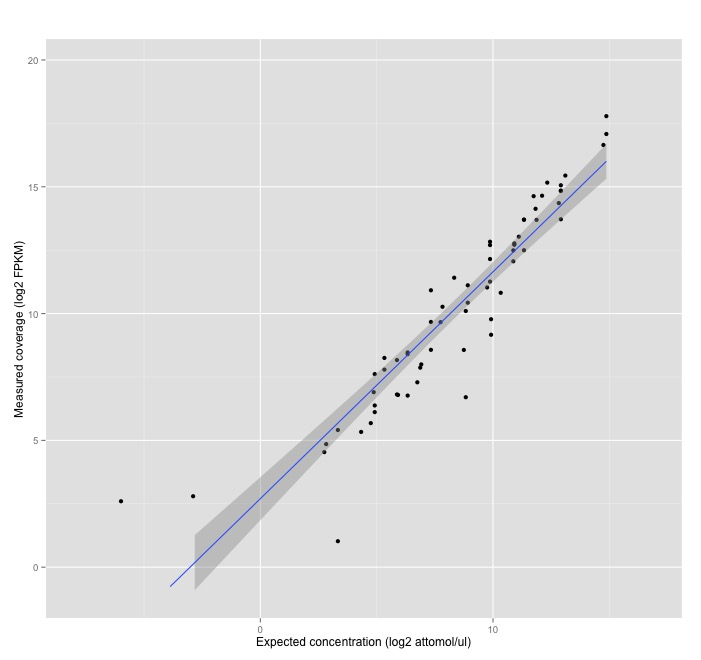
\includegraphics{5.jpeg}

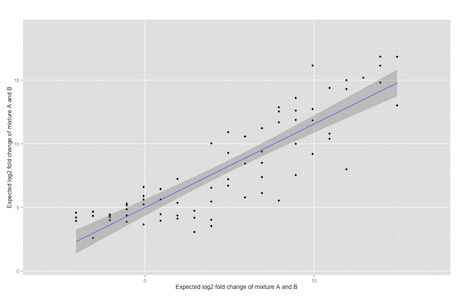
\includegraphics{3.jpeg}

\end{document}
